\section{Arkitektur}\label{sec:arkitektur}
Eftersom vi ikke har fundet et eksisterende arkitekturmønster der kan tilgodese vores krav opstillet i \cref{arkitekturkrav}, har vi konstrueret vores egen arkitektur der forsøger at tilgodese kravene bedst muligt.
Arkitekturen er lavet ud fra ideen om at apps på android kan kontakte hinanden igennem android systemet. 
Det er altså muligt for en hovedapplikation at starte en service der ligger i en anden applikation.
Dette udnytter vi ved at alle moduler bliver pakket i en selvstændig app som også tjener det formål at give den modulære tilgang vi leder efter. 
Ved at lave en adgangsbeskyttet database vil det være muligt for moduler at få adgang til data fra andre moduler.
Til sidst vurderes det også at en central bestyrende enhed er nødvendig for at have et bindeled mellem alle de selvstændige apps det blev valgt at installere.

\section*{Opbygning}
Den overordnede arkitektur er opbygget af fire komponenter: \textit{manager}, \textit{moduler}, \textit{DB access} og \textit{DB}.

Det første udkast af arkitekturen kan ses på \cref{arkitektur_udkast_1}.
\begin{figure}[h]
	\centering
	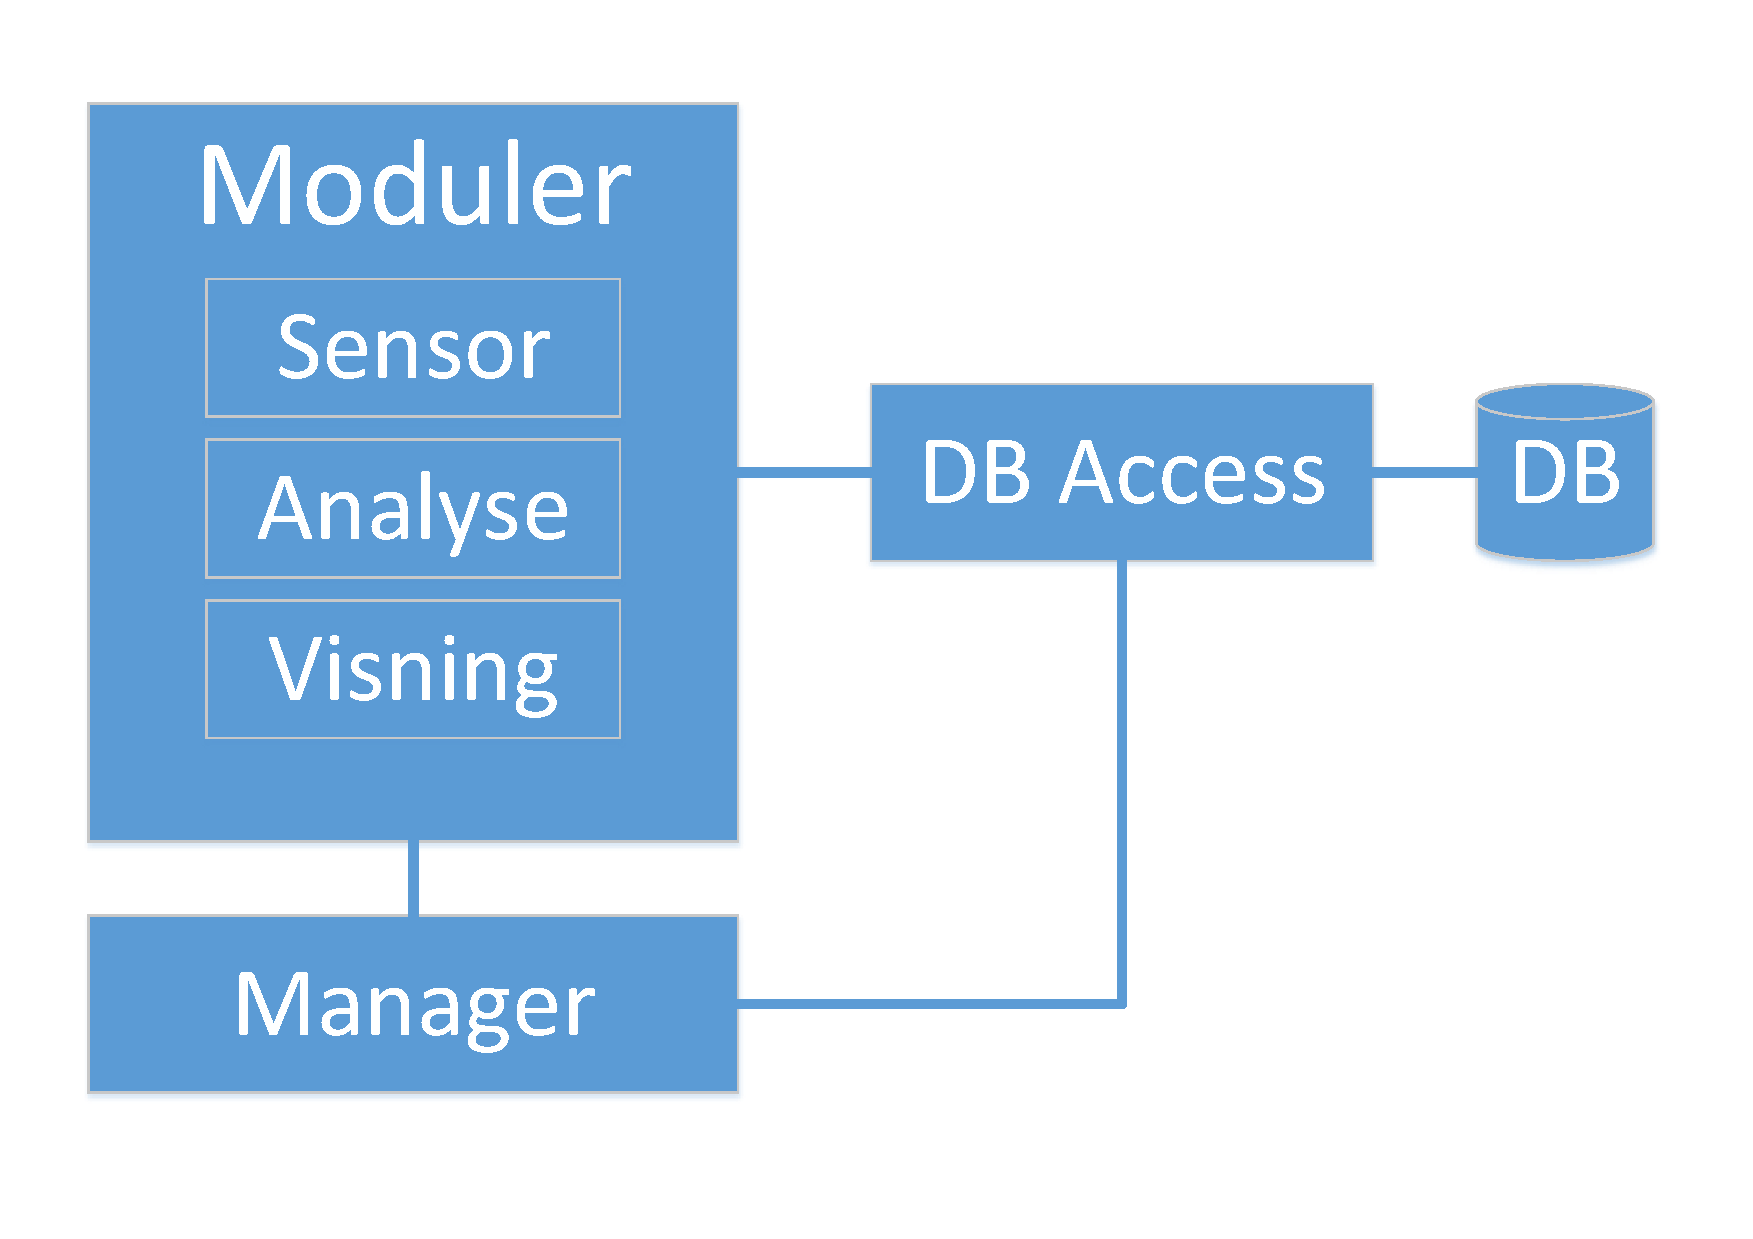
\includegraphics[width=0.9\textwidth]{ArkitekturVisio}
	\caption{Første udkast til arkitektur.}
  \label{arkitektur_udkast_1}
\end{figure}

Herunder gives en beskrivelse af hver af de fire komponenter.
Komponenterne beskrives i rækkefølge af deres indbyrdes afhængighed, således at forståelsen af hver komponent kun afhænger af det læste.

\subsection*{DB}
Denne komponent administrerer data for systemets forskellige moduler.
Data opbevares i en række tabeller i et relationelt database system.
Hvert modul har mulighed for at definere egne tabeller, der alle gemmes i \textit{DB} komponenten.

Til dette projekt er valgt en SQLite database da denne er standard i Android.


\subsection*{DB Access}
Denne komponent styrer adgangen til \textit{DB} komponenten så det sker på en ensrettet måde.
Da vi arbejder på en mobil platform er det værd at tage højde for lagerstyring og abstraktion derover.
Da der er begrænset plads på en smartphone kan det blive relevant at lagre noget af det indsamlede data i skyen.
Men det kan være nyttigt at abstrahere over hvor data indsamles og lagres, og er fint i tråd med de krav om generalitet og fleksibilitet for platformen.

Da det er intentionen, at eksterne udviklere skal kunne udvikle moduler til systemet, er det nødvendigt at sørge for at moduler har adgang til kun at skrive til deres egen database og samtidig læse fra alle andres database.
På denne måde forhindres det at eksterne moduler korrumperer andre modulers data, enten ved et uheld eller med vilje.

\paragraph{Design} 
For at imødekomme kravene om både at give ensrettet adgang til moduler og stille garantier om adgangsrettigheder har vi undersøgt eksisterende mønstre der vil kunne opfylde disse krav.

\subparagraph{Facade}
For at kunne give en ensrettet interface til moduler tager vi inspiration i det strukturelle \textit{facade} design mønster.
Facade er et design mønter der tilbyder et simpelt interface til et komplekst subsystem \citep{DATGANGOFFOUR}. 
Det er et middel til at få en løsere kobling mellem et system og klienterne der bruger systemet.
Dette gøres ved at opstille en facade mellem klienterne og subsystemet.
Facaden sikrer et ensartet interface til brug af subsystemerne, men hvor man abstraherer over disse.
At implementere dette sikrer også større modularitet idet ændringer i subsystemerne ikke kræver ændring i klienterne, da de blot bruger facaden der kan justere for disse ændringer.

Af denne årsag vælges der at bruge facade designmønstret til at abstrahere over lagringen af data.
Implementationen af dette mønster er udført ved at udnytte androids indbyggede \textit{Content Provider} konstruktion.
En Content Provider indkapsler en mængde af struktureret data, hvilket i vores tilfælde er det data som DB Access råder over \cite{contentprovider}.
\stefan{mere detalje?}

\subparagraph{Observer}
For at moduler kan tilgå hinandens data uden at have adgang til at tilføje eller ændre i det har vi brug for en model til at dele data.

En overvejelse har været at bruge observer mønstret til dette.
Med observer mønstret kan man hver gang der er nyt data sende opdateringen ud til alle de moduler der har brug for dataen \cite[p.~244]{gamma1994design}.

Ved brug af dette mønster vil hvert modul der abonnerer på en datakilde kunne udføre sine beregninger med det samme når dataen er tilgængelig.
Det betyder på den anden side at det ikke er muligt for modulet selv at bestemme hvornår tunge beregninger skal udføres.
Hvis et modul skal udføre tunge beregninger vil det være fordelagtigt at kunne udføre disse når brugeren ikke bruger telefonen, eventuelt om natten når telefonen alligevel er sat til strøm.
Vi har derfor valgt ikke at bruge observer mønstret til deling af data.

\subparagraph{Sikkerhed}
Udover at være ensrettet skal \textit{DB Access} også sørge at et komponent kun kan skrive til sine egne tabeller, men samtidig have mulighed for at læse fra andre modulers tabeller.
Denne del af systemet er ikke implementeret.

\paragraph{Fremtidig udvikling}
På nuværende tidspunkt er sikkerhedsdelen ikke implementeret, og alle moduler kan derfor både læse og skrive til alle databasetabeller.
For at undgå at en udvikler kan lave et modul der ødelægger data for et andet modul er dette nødvendigt.
Vi forestiller os at der skal laves en nøgleudveksling mellem manager og modul når et modul installeres, så manageren kan kende forskel på moduler og derved begrænse skriveadgang til modulet der har oprettet tabellen.
\stefan{skriv eventuelt også i refleksion}

Det udviklede system anvender en database placeret på selve mobiltelefonen og er dermed begrænset af de muligheder der er for lagring på den enkelte enhed.
Da der er begrænset plads på en mobiltelefon (se \cref{eksperimenter}) vil denne løsning muligvis udløse en række problemer.
Det vil derfor være en naturlig udvidelse af DB Access skal sørge for at uploade data til et eksternt lager når dataen ikke er nødvendig at lagre på telefonen mere.
På denne måde begrænser man systemets pladsforbrug, og kan samtidig foretager analyser på al dataen hvis en ny analyse installeres på systemet.
Denne ændring kan desuden udføres uden at kræve ændringer i andre moduler end DB Access da Facade mønsteret er taget i brug.

\subsection*{Moduler}
Moduler komponenten i arkitekturen befinder sig i et lag for sig selv.
Moduler indeholder applikationens hovedfunktionalitet og er ansvarlig for indsamling af data, bearbejdelse af data og visning af data.

\paragraph{Design}
Til hvert enkelt modul hører en modulbeskrivelse (se \cref{modul_definition}) der beskriver modulets afhængigheder af andre moduler samt hvordan det skal administreres i systemet.
Denne administration består til dels i en definitioner af de tabeller modulet har behov for at få oprettet i \textit{DB} komponenten.

Modullaget inddeles yderligere i tre konceptuelle lag: \textit{sensor}-, \textit{analyse}- og \textit{visnings}moduler.

Nedenstående beskriver intentionerne bag de forskellige modultyper og deres opgave.

\subparagraph{Sensor}
\textit{Sensor}laget indeholder moduler der indsamler data fra telefonens (eller tilbehør dertil) forskellige sensorer og applikationer.
Der påføres kun et minimum af behandling på indsamlede data (eksempelvis komprimering) således at data kan indsamles kontinuert uden stort energi-behov.
Derudover for at have mulighed for at lave meningsfulde analyser skal alt logget data gemmes i \textit{DB} i rå eller komprimeret form.
Det vil sige at komprimering skal være tabsfri og at eventuelle fejlmålinger bør markeres som sådan i den pågældende data tabel.

Et eksempel på et sensormodul er indsamling af data fra accelerometret.
Modulet får data fra accelerometret og gemmer det i sin database. 
For ikke at gemme unødvendige mængder data vil modulet kun gemme et datapunkt når det er forskelligt fra det forrige målte punkt.

\subparagraph{Analyse}
\textit{Analyse}laget indeholder moduler der bruger data fra et antal sensormoduler samt eventuelle andre analysemoduler.
Herefter udføres en analyse af det indsamlede data med \textit{''forståelig information''} som resultat.
I denne process vil der kunne forekomme tab af data.
Herved opnås en opsummering af det indsamlede data, der skaber værdifuld information for brugeren.
Som en del af et analysemoduls beskrivelse findes en beskrivelse af hvilken information man kan få fra modulet.
Denne information anvendes af visningsmodulerne.

Der kan ved analyse af sensordata anvendes flere ressourcer, da analysen typisk vil kunne udføres på større mængder indsamlede data få gange dagligt.
Eksempelvis kan analysen foretages om natten hvor telefonen kan sættes til opladning.

Et eksempel på et analysemodul kan være et søvnanalyse modul der bruger førnævnte accelerometer data til at undersøge en sovendes søvn.
Dette modul vil bruge flere sensormoduler til sin analyse og vil muligvis bruge accelerometerdata fra både en smartphone og et smart watch.

\subparagraph{Visning}
\textit{Visnings}laget indeholder moduler der visualiserer analyserede data.
Som en del af et visningsmoduls beskrivelse findes en beskrivelse af hvilken information modulet accepterer.
Hvis denne beskrivelse stemmer overens med et analysemodul, kan den enkelte visning anvendes på den enkelte analyse.

Et eksempel på et visningsmodul er et modul der visualisere de resultater som føromtalte søvnanalyse har fundet frem til.
Dette kunne være en graf der fortæller hvor dyb søvn man har været i, eller en simpel farvet indikator hvis farve viser hvor godt man har sovet de sidste par dage.

Eksempelvis vil et accelerometer \textit{sensor}modul kunne anvendes af et søvn \textit{analyse}modul der viser resultatet i et graf \textit{visnings}modul.

Skulle man her ønske en anden fortolkning af accelerometerets data kan et andet analysemodul anvendes.
Sammensætningen af analyse- og visningsmoduler sker ved en beskrivelse af deres grænseflade.
Moduler med fælles grænseflade vil kunne kombineres.
Det vil sige at der kan anvendes flere forskellige visningsmoduler til det samme analysemodul, givet at de er kompatible.
Tilsvarende kan det samme visningsmoduler anvendes til flere forskellige analysemoduler.

\paragraph{Fremtidig udvikling}

\stefan{ideer?}

\subsection*{Manager}\label{subsec:arkitektur-Manager}
Manager komponenten kan siges at være grænsefladen mellem bruger og moduler.
Den står for at administrere de installerede moduler ud fra de beskrivelser der er givet for de enkelte moduler.
Denne administration indebærer blandt andet oprettelse af de database tabeller hvert modul har bedt om i sin beskrivelse, samt start og stop af sensor- og analysemoduler.
Sidstnævnte sker ud fra definitioner givet i beskrivelserne af de enkelte moduler.
Desuden er det også gennem manageren brugeren for vist den information de leder efter.

\paragraph{Design}
Ved at sammenholde visninger og analyser kan manageren beskrive for brugeren hvilke data der kan fremvises og med hvilke visninger det kan ske.
Manageren har desuden en prædefineret brugerflade der anvender ovenstående kombinationer til at vise brugeren de relevante informationer.

Manager komponenten indeholder desuden et JSON skema for hver modul-type i moduler komponenten.
Disse definitioner beskriver formatet for eventuelle nye moduler man måtte ønske at føje til systemet.
\stefan{et eller flere skemaer? Muligvis har views anderledes skema, men analyse og sensorer har det samme}


\paragraph{Fremtidig udvikling}

\stefan{ideer?}

